\documentclass{standalone}
\usepackage{tikz}
\usepackage{ctex,siunitx}
\setCJKmainfont{Noto Serif CJK SC}
\usepackage{tkz-euclide}
\usepackage{amsmath,mhchem}
\usetikzlibrary{patterns, calc}
\usetikzlibrary {decorations.pathmorphing, decorations.pathreplacing, decorations.shapes,}
\begin{document}
\small
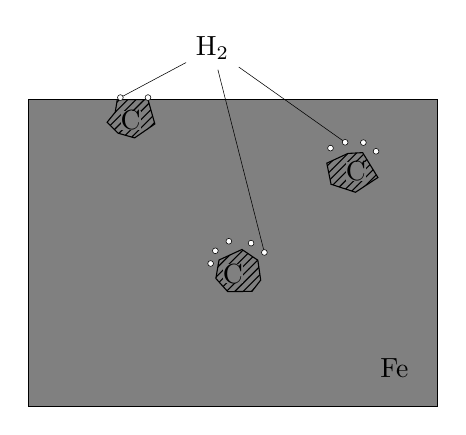
\begin{tikzpicture}[>=stealth,scale=1.3]
  \draw[fill=gray](-2,3)rectangle(2,0)node[above left=10pt]{\ce{Fe}};
  \node (h2) at (-0.2,3.5){\ce{H2}};
  \draw[pattern=north east lines](-1.130,3.000)--(-1.150,2.877)--(-1.229,2.779)--(-1.122,2.672)--(-0.961,2.626)--(-0.763,2.762)--(-0.830,3.000)--cycle( 0.088,1.536)--(-0.136,1.433)--(-0.167,1.253)--(-0.051,1.124)--( 0.186,1.127)--( 0.271,1.237)--( 0.243,1.431)--cycle
(1.123,2.474)--(0.917,2.379)--(0.958,2.173)--(1.197,2.095)--(1.416,2.239)--(1.267,2.482)--cycle;
  \node at (-1,2.8)[inner sep=0pt,fill=gray] {\ce{C}};
  \node at (0,1.3)[inner sep=0pt,fill=gray] {\ce{C}};
  \node at (1.2,2.3)[inner sep=0pt,fill=gray] {\ce{C}};
  \draw[very thin](-1.1,3.02)--(h2);
  \draw[very thin](0.307,1.507)--(h2);
  \draw[very thin](1.096,2.583)--(h2);
  \foreach \x/\y in {
    -0.218/1.399,
    -0.172/1.523,
    -0.040/1.616,
    0.177/1.598,
    0.307/1.507,
    0.953/2.526,
    1.096/2.583,
    1.274/2.580,
    -1.1/3.02,
    -0.83/3.02,
    1.398/2.495%
  }
  {\draw[very thin,fill=white] (\x,\y) circle(0.8pt);}
\end{tikzpicture}
\end{document}